\documentclass{beamer}
\usepackage{color,amsmath}
\usepackage{subfigure}
\usepackage{booktabs}
\usepackage{framed}
\usepackage{comment}
\usepackage{cancel}

\usetheme[progressbar=frametitle]{metropolis}
\usepackage{appendixnumberbeamer}

\usepackage[scale=2]{ccicons}

\usepackage{pgfplots}
\usepgfplotslibrary{dateplot}

\usepackage{xspace}
\newcommand{\themename}{\textbf{\textsc{metropolis}}\xspace}



\def\vf{\vfill}

%%%%%%%%%%%%%%%%%%%%%%%%%%
\title{Why SICSS?}
\subtitle{Bamberg Summer Institute in Computational Social Science}
\author{Carsten Schwemmer, University of Bamberg}
\institute{\textit{Many thanks to Chris Bail for providing material for this lecture}}
\date{2019-07-29}
\vfill

\begin{document}
%%%%%%%%%%%%%%%%%%%%%%%%%%
\maketitle
%%%%%%%%%%%%%%%%%%%%%%%%%%

\section{Why SICSS?}

\begin{frame}{Big problems in the world}

\begin{center}
	
\includegraphics[width=1.0\textwidth]{figures/cambridge.jpg}
\end{center}

\end{frame}

\begin{frame}{Our field is growing}

\begin{center}
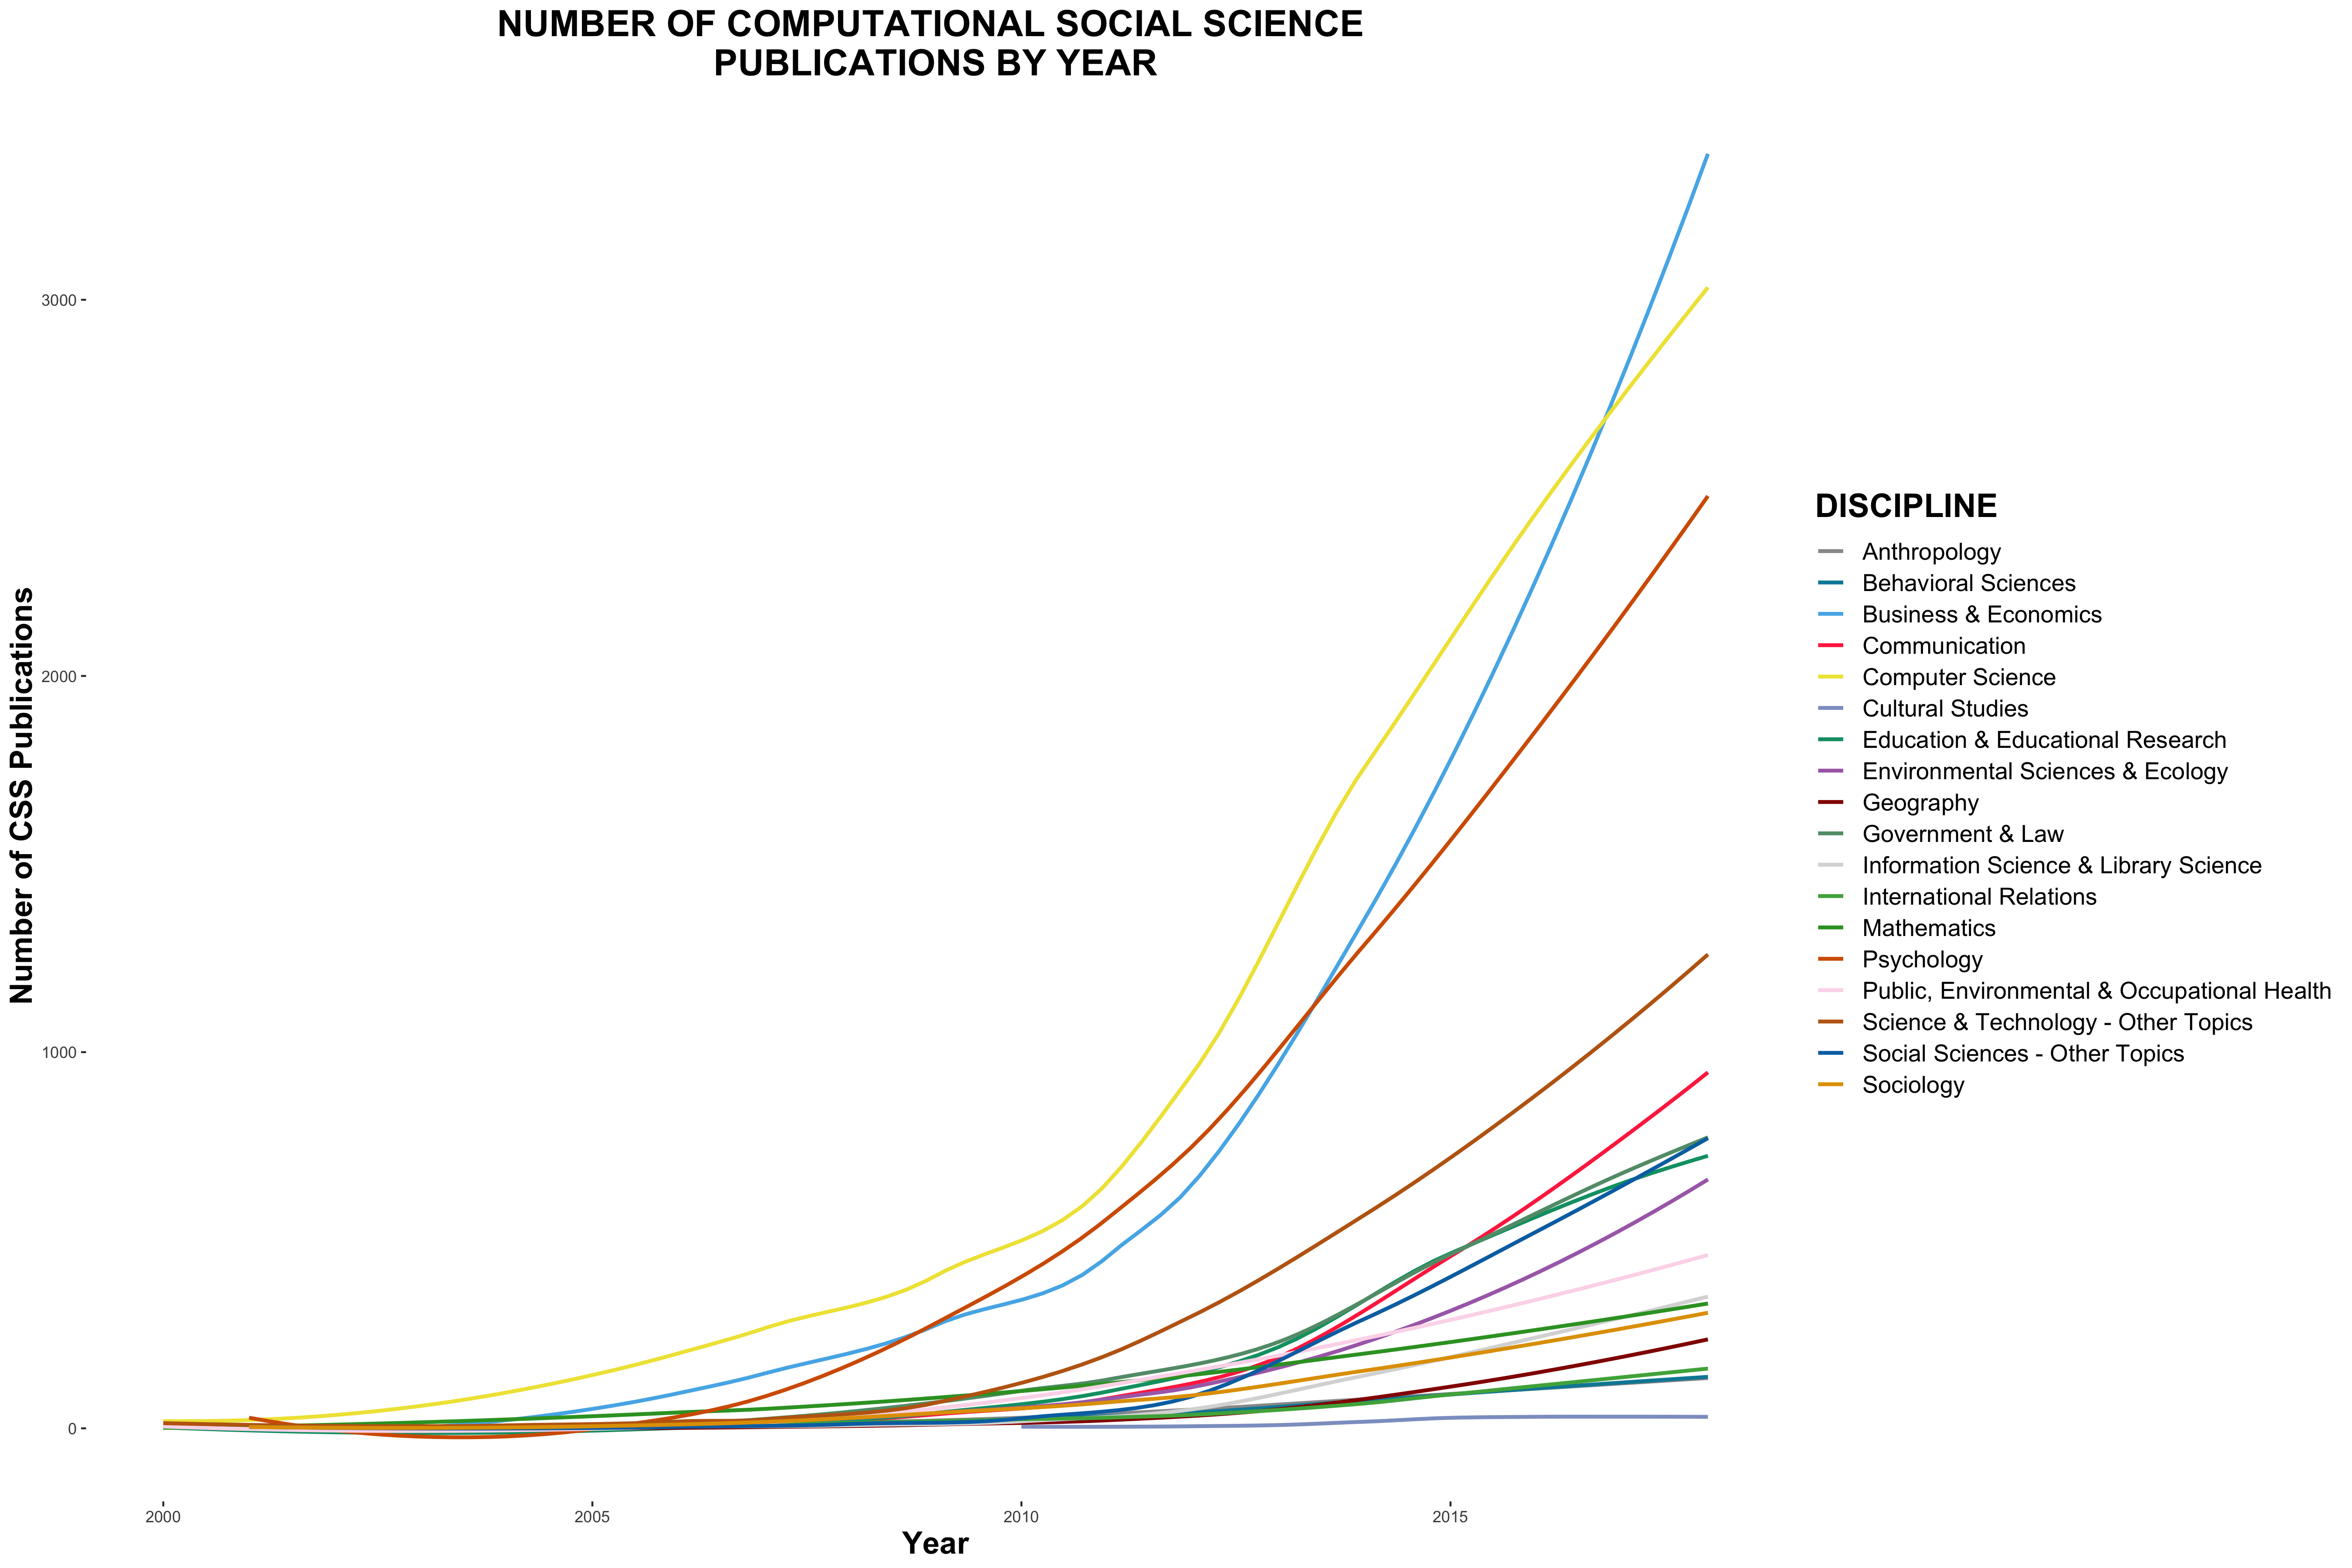
\includegraphics[width=1.0\textwidth]{figures/ss_disciplines_time.jpg}
\end{center}

\vf
\tiny{\url{https://www.chrisbail.net/post/mapping-computational-social-science}}


\end{frame}

\begin{frame}{Our field is interdisciplinary}

\begin{center}
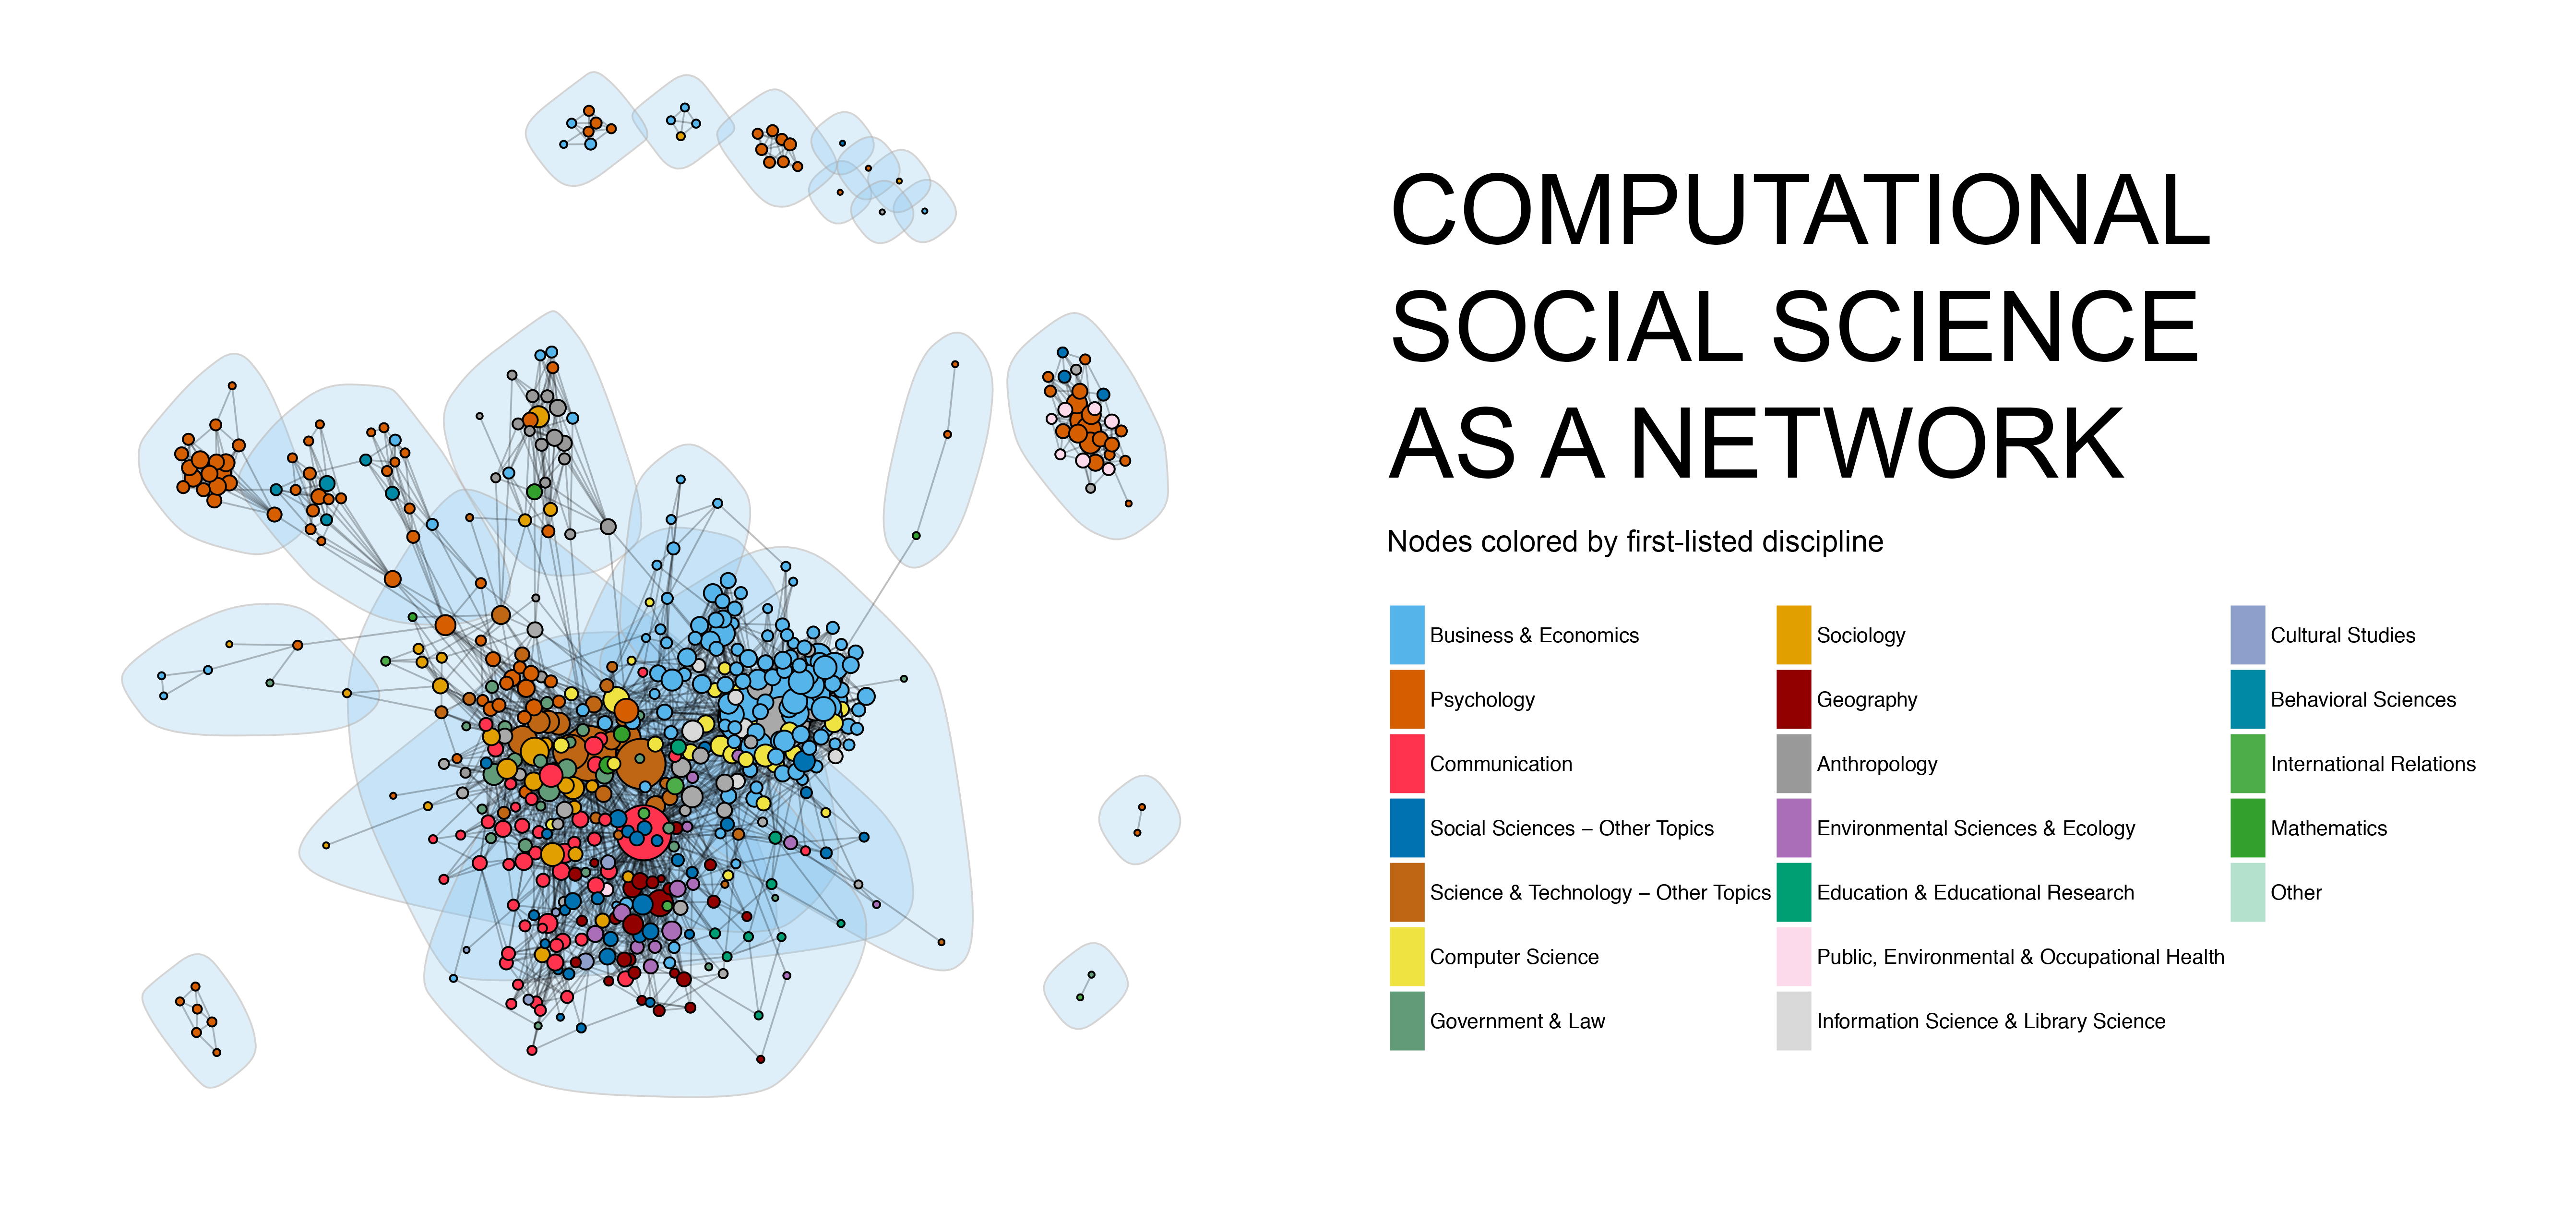
\includegraphics[width=1.0\textwidth]{figures/colore_by_nodes_arial.png}
\end{center}


\vf
\tiny{\url{https://www.chrisbail.net/post/mapping-computational-social-science}}

\end{frame}

\begin{frame}{Training opportunities are rare}

\begin{center}

\includegraphics[width=1.0\textwidth]{figures/code.jpg}
\end{center}

\end{frame}

\begin{frame}{SICSS as a possible solution}

\begin{center}

\includegraphics[width=0.6\textwidth]{figures/sicss_logo.png}
\end{center}

\end{frame}

\begin{frame}{Goal 1: provide state-of-the-art training}

\begin{center}

\includegraphics[width=1.0\textwidth]{figures/code.jpg}
\end{center}

\end{frame}

\begin{frame}{Goal 2: challenge disciplinary divides}

\begin{center}
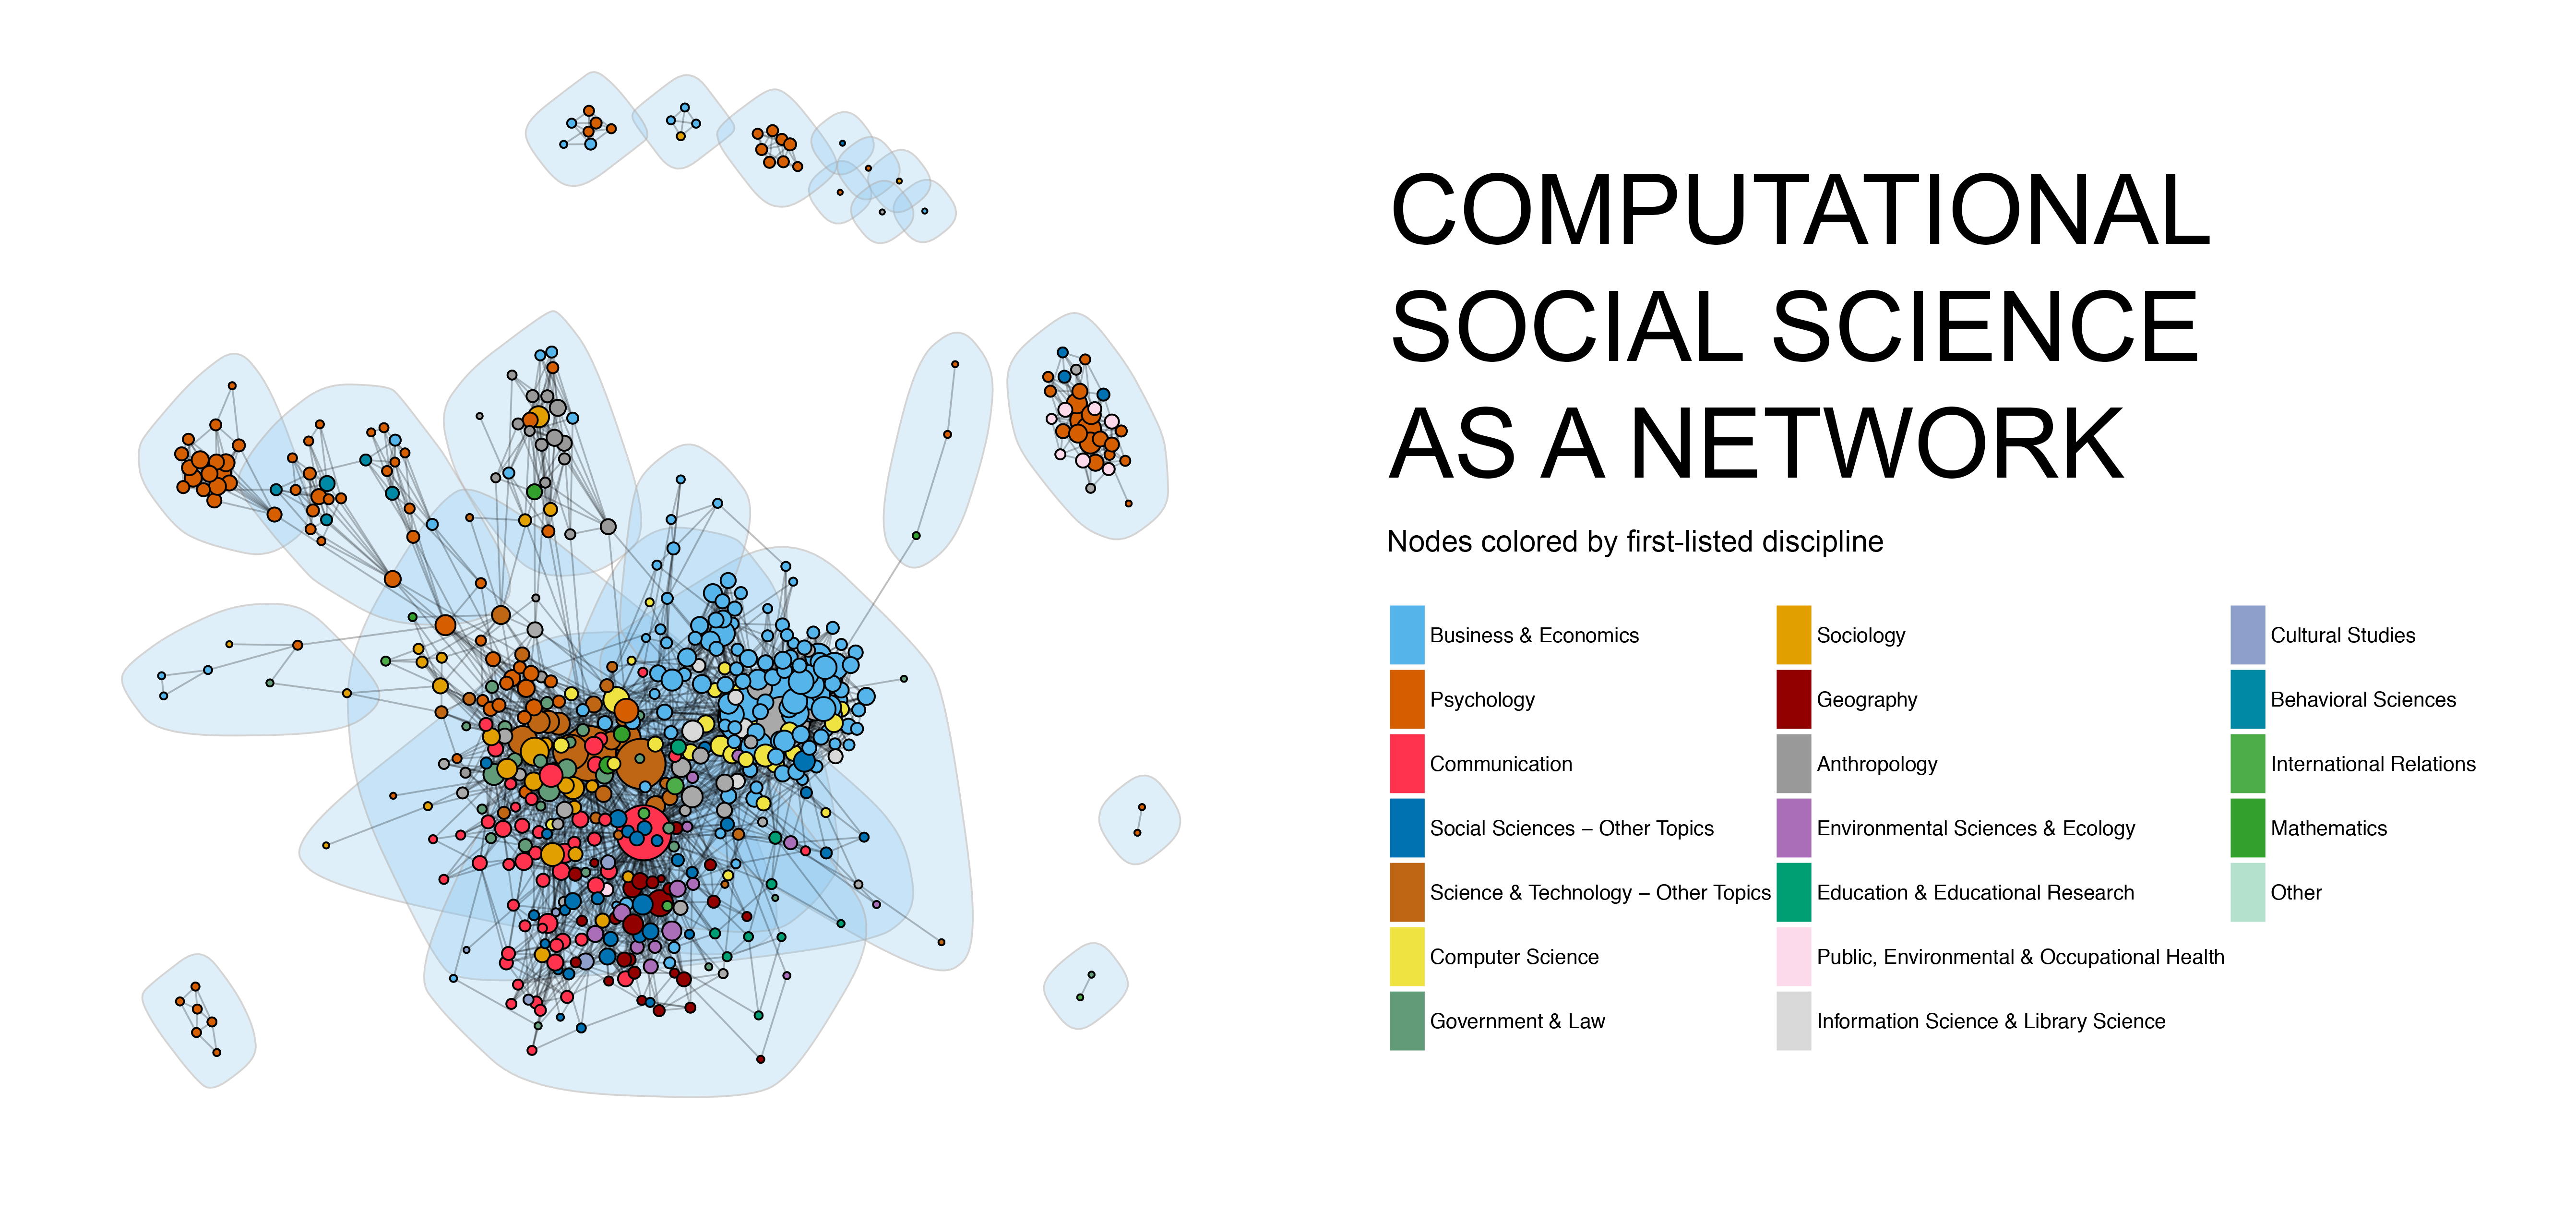
\includegraphics[width=1.0\textwidth]{figures/colore_by_nodes_arial.png}
\end{center}



\end{frame}

\begin{frame}{Goal 2: challenge disciplinary divides}

\begin{center}
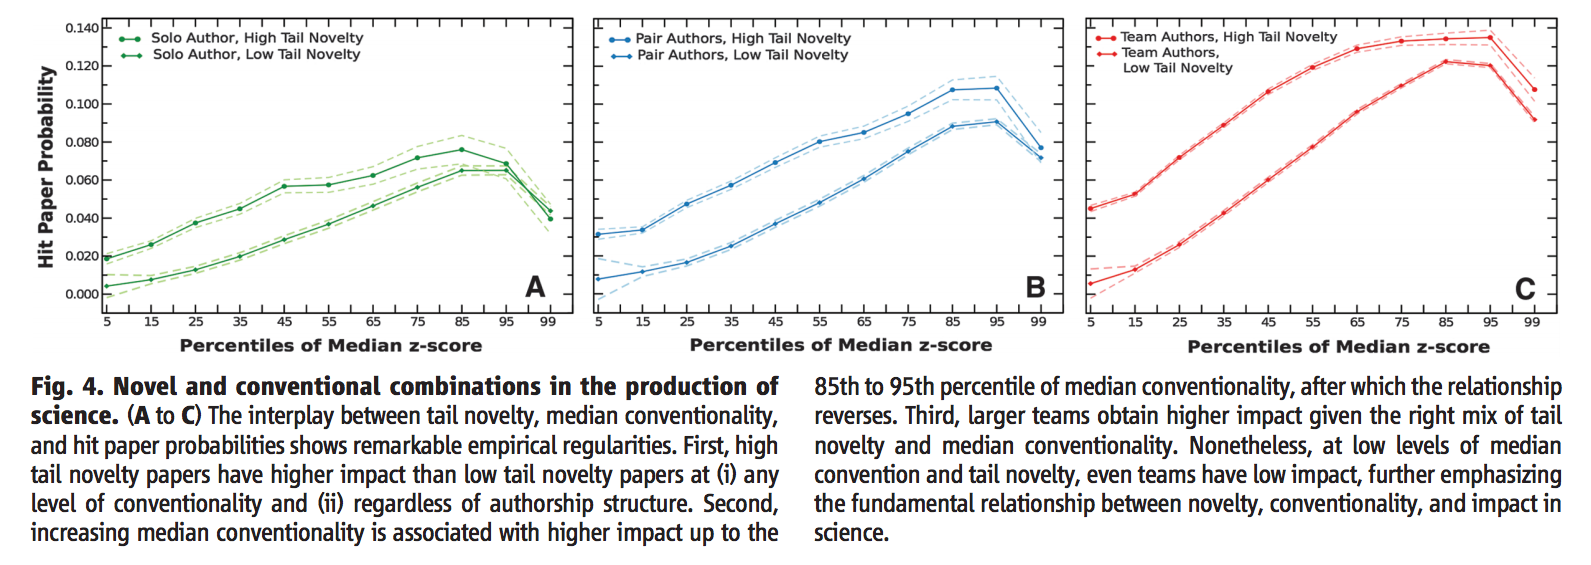
\includegraphics[width=1.0\textwidth]{figures/impact.png}
\end{center}

\vf
\tiny{\url{https://link.springer.com/chapter/10.1007/978-3-319-45023-0_12}}
\end{frame}

\begin{frame}{Goal 3: reach a broad audience}

\begin{center}
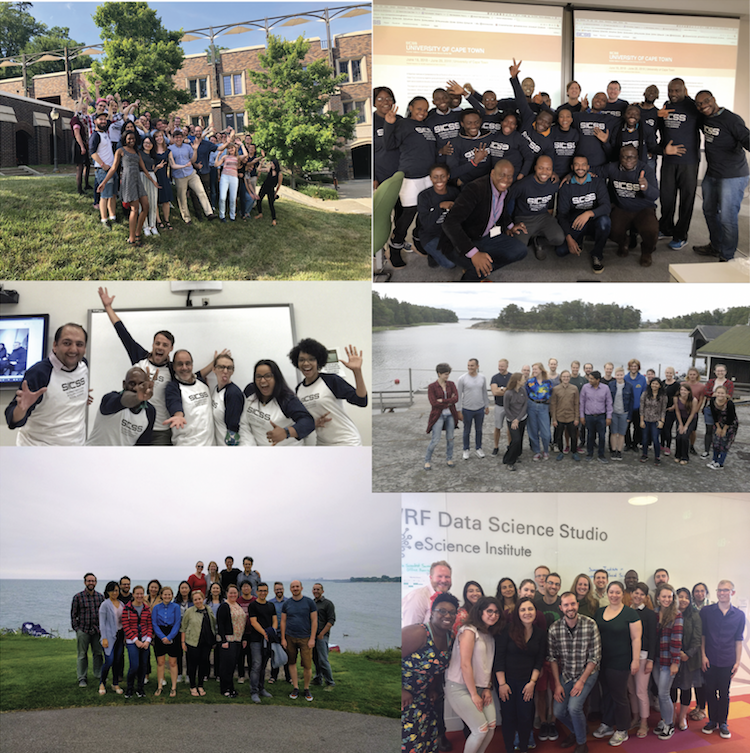
\includegraphics[width=0.65\textwidth]{figures/sicss_collage.png}
\end{center}

\end{frame}

\begin{frame}{Goal 3: reach a broad audience}

\begin{center}
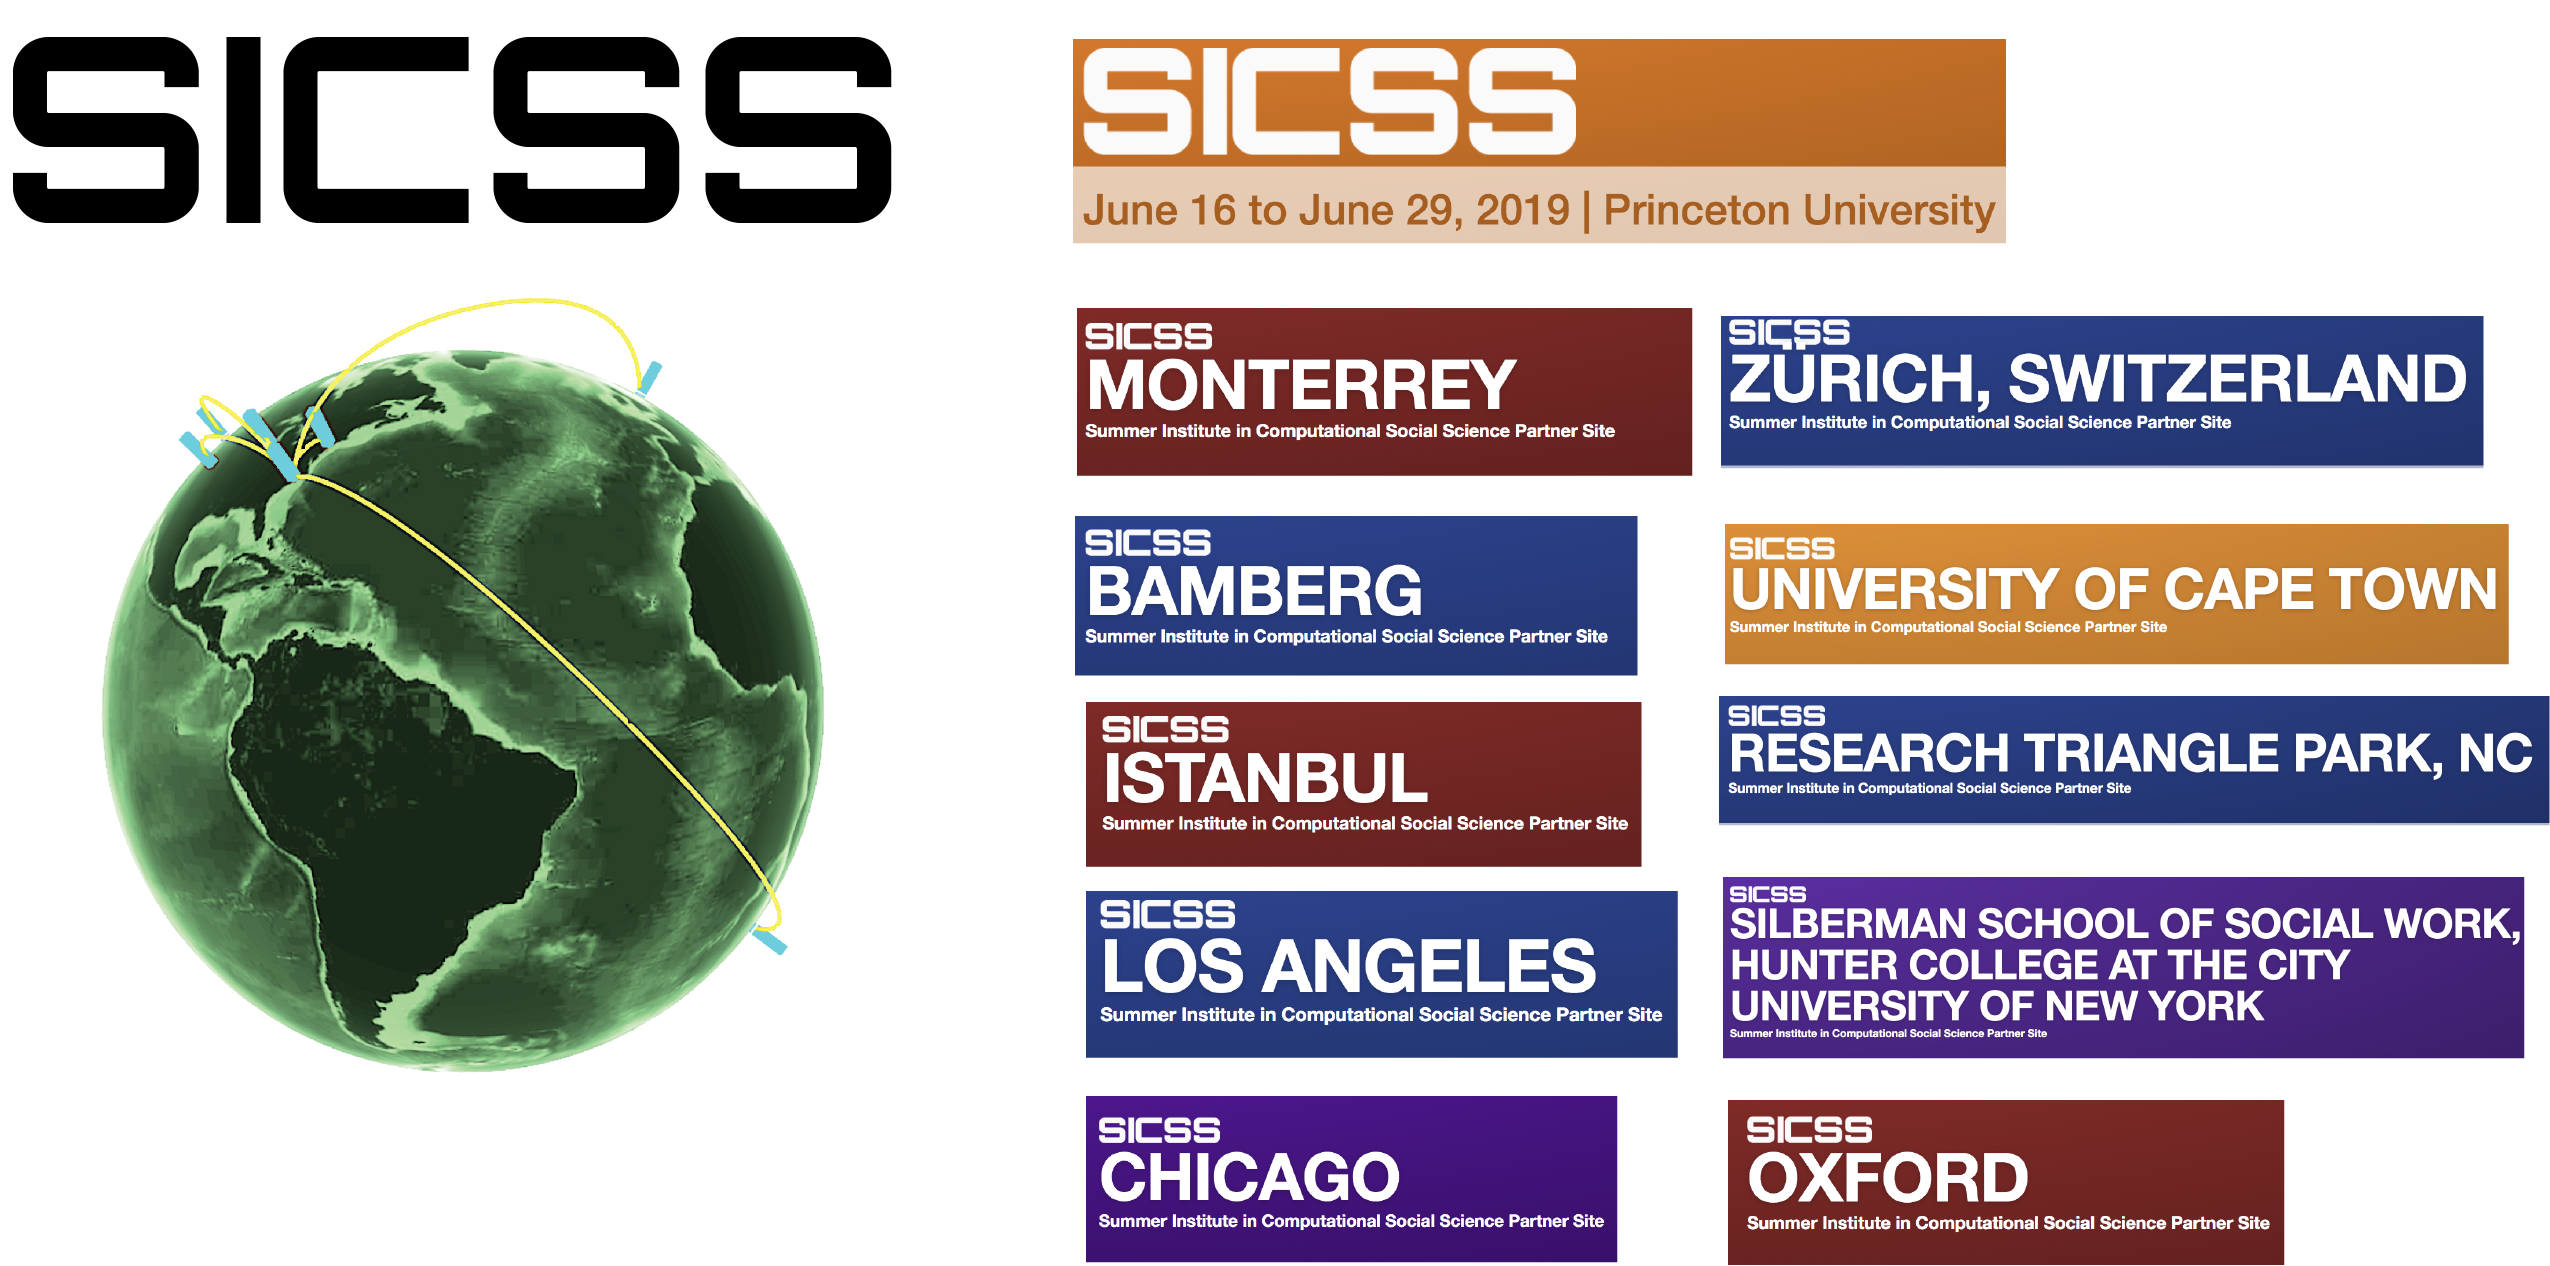
\includegraphics[width=1.0\textwidth]{figures/sicss_world.png}
\end{center}

\end{frame}

\begin{frame}{Goal 4: open-source}



All materials for lectures and group activities (slides, images, R Markdown files, data) will be available on Github:

\url{https://github.com/compsocialscience/summer-institute/tree/master/2019/bamberg/materials}

\begin{center}
	
\includegraphics[width=0.8\textwidth]{figures/sicss_bamberg.png}
\end{center}

\end{frame}

\begin{frame}{Goal 5: teach the teachers}

\begin{center}
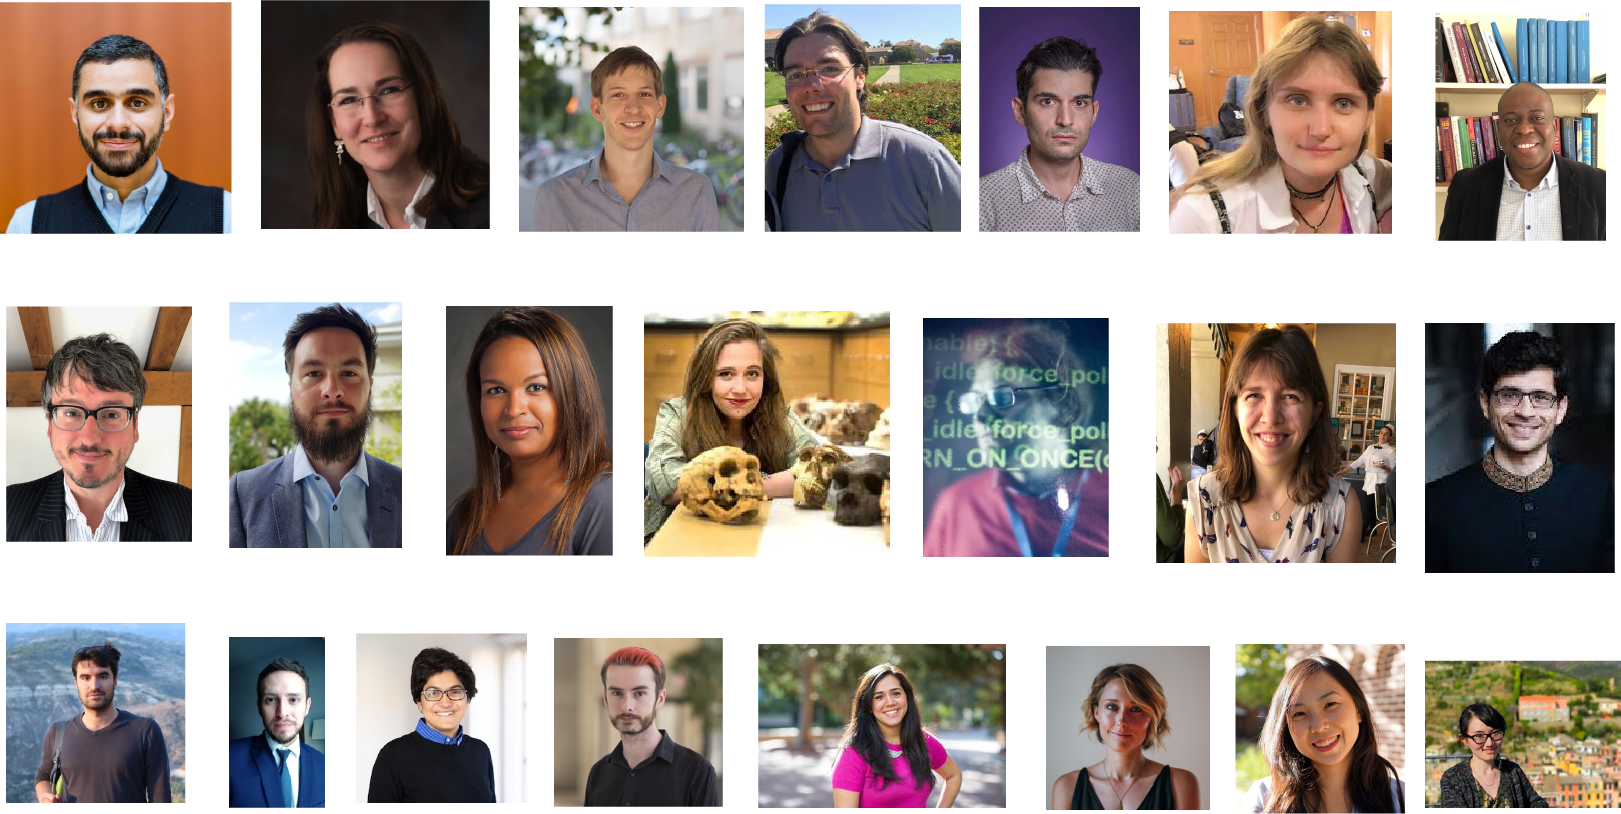
\includegraphics[width=1.0\textwidth]{figures/alumni_leaders.png}
\end{center}

\end{frame}

\begin{frame}{Goal 6: create a diverse community}

\begin{center}
\includegraphics[width=1.0\textwidth]{figures/sicss_mosaic.png}
\end{center}

\end{frame}

\section{How SICSS works}

\begin{frame}{Schedule}

\begin{center}
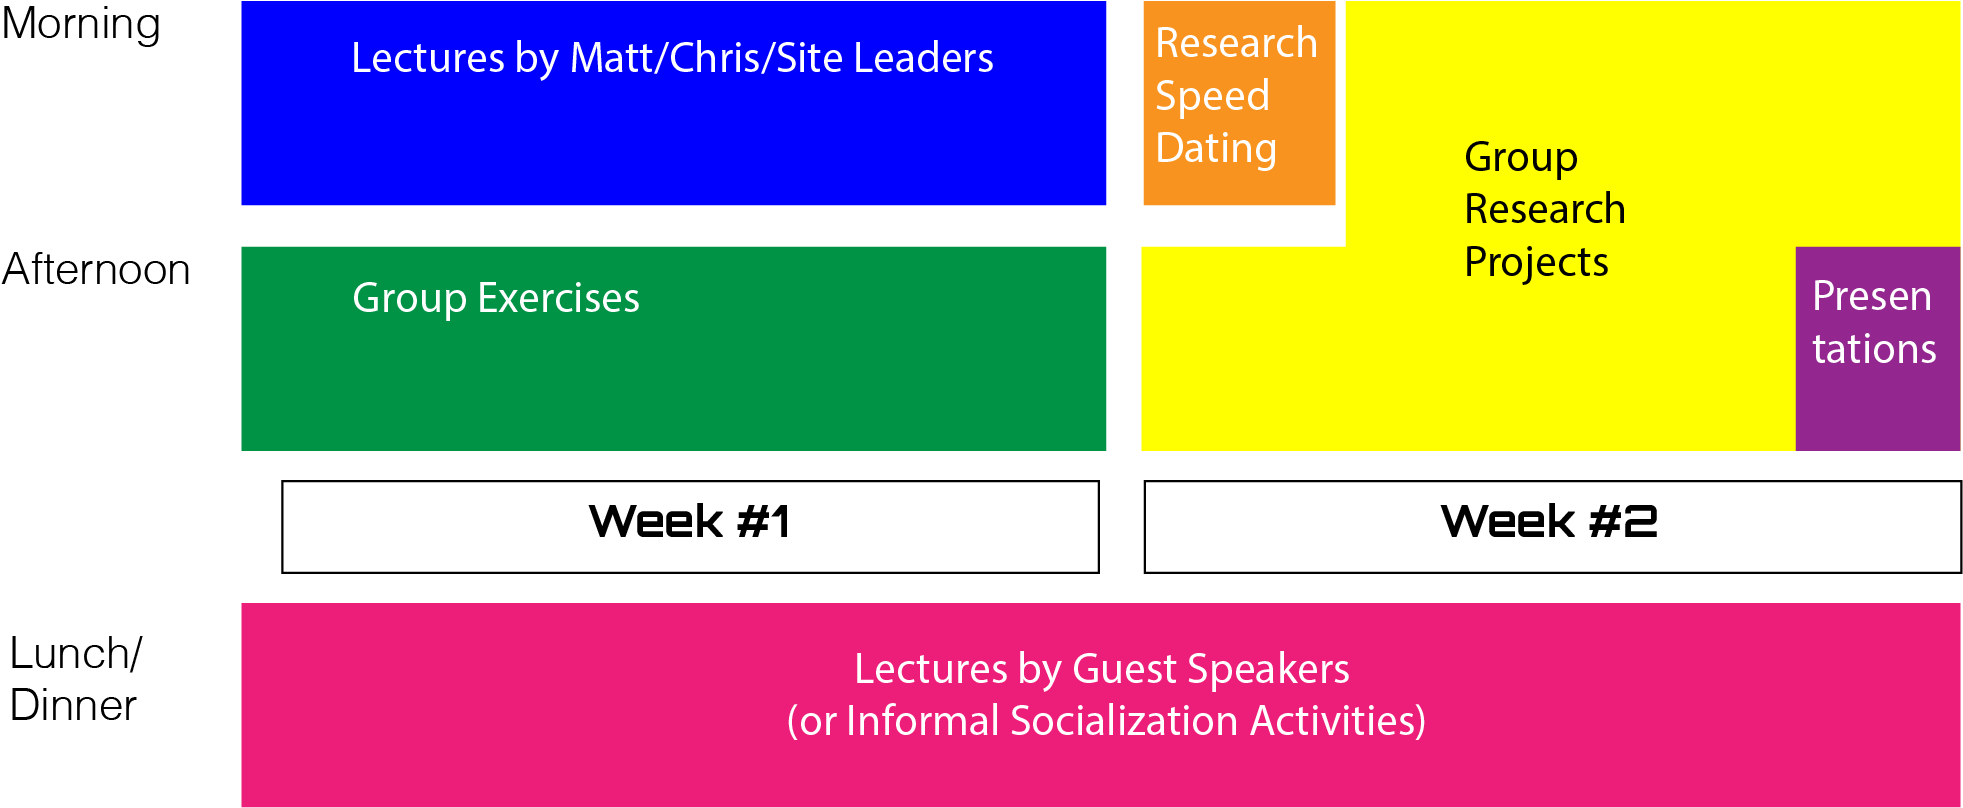
\includegraphics[width=1.0\textwidth]{figures/SICSSAnatomy.png}
\end{center}

\end{frame}


\begin{frame}{Lectures}

\begin{center}
\begin{tabular}{ c|c|c } 
\hline
\textbf{Day} & \textbf{Topic} & \textbf{Lecturer} \\
\hline
Monday & Intro/Ethics & Carsten \\ 
Tuesday & Collecting Digital Trace Data & Carsten \\ 
Wednesday & Social Network Analysis & Oliver Posegga\\ 
Thursday & Automated Text Analysis & Carsten \\ 
Friday & Surveys in the Digital Age & Matt (video lecture)\\ 
Saturday & Field Experiments & Matt (video lecture)\\ 

\hline
\end{tabular}
\end{center}

\end{frame}

\begin{frame}{Accessing materials}

Go to this site: \\
\url{https://compsocialscience.github.io/summer-institute/2019/bamberg/\#schedule}

\end{frame}


\begin{frame}{Guest speakers}



\begin{center}
\begin{tabular}{ c|c|c } 
\hline
\textbf{Day} & \textbf{Mode} & \textbf{Speaker} \\
\hline
Monday (week 1) & Local & Andreas Jungherr\\ 
Tuesday (week ) & Video & Deen Freelon \\ 
Wednesday (week 1) & Local & Fariba Karimi \\ 
%\cancel{Thursday (week 1)} & \cancel{Video} & \cancel{Justin Grimmer} \\ 
Friday  (week 1)& Local & Ridhi Kashyap\\ 
Monday  (week 2)& Local & Martijn Schoonvelde\\ 
Tuesday (week 2)& Local & Milena Tsvetkova \\ 

\hline
\end{tabular}
\end{center}

All of our local guest speakers will be available for office hours. Please let us know as soon as possible if you want to talk to them.

\end{frame}


\begin{frame}{Group projects}

\begin{center}
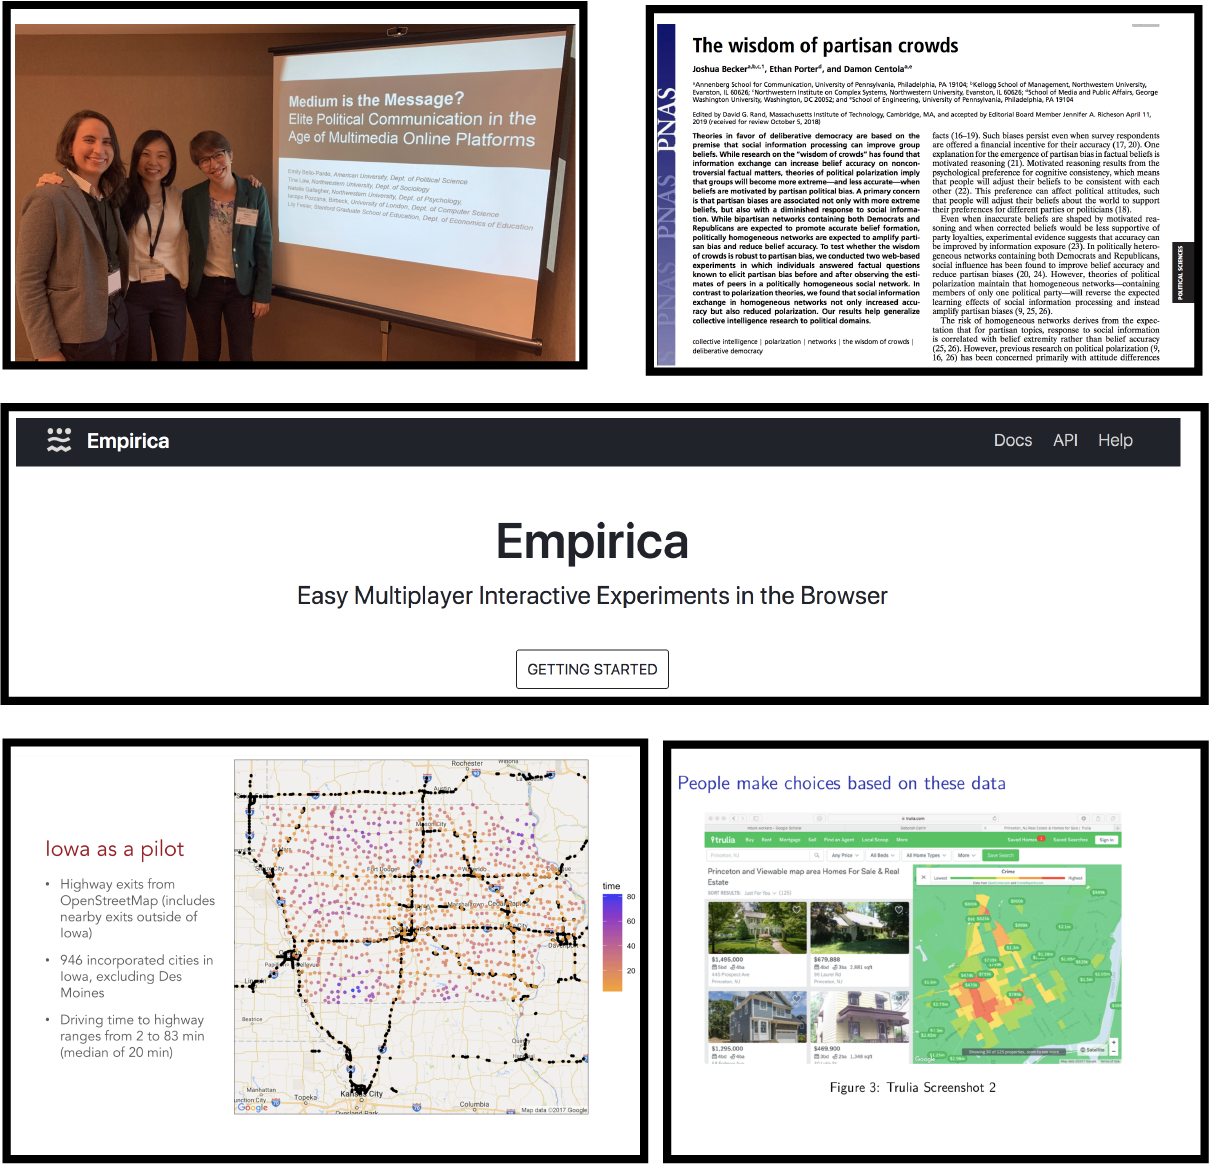
\includegraphics[width=0.75\textwidth]{figures/2019_group_projects.png}
\end{center}

\end{frame}


\begin{frame}{Your responsibilities}

\begin{itemize}
\item openness
\item patience
\item togetherness
\item generosity
\end{itemize}

\end{frame}

\begin{frame}{Feedback}

Link to a general SICSS feedback form (shared among partner institutes)
\url{https://forms.gle/kZsrPrmu66LPqQME9}

\vspace{2mm}
For the first week, we will also have daily feedback forms specific to SICSS Bamberg

\end{frame}


\begin{frame}[standout]

\begin{center}
\LARGE
Questions?
\end{center}

\end{frame}

\end{document}